\documentclass[a4paper,12pt]{article}

\usepackage[T2A]{fontenc}
\usepackage[utf8]{inputenc}
\usepackage[english,russian]{babel}
\usepackage{amsmath, amsfonts, amsthm}
\usepackage{listings}
\usepackage{enumerate}
\usepackage{float}
\usepackage{graphicx}
\usepackage{nameref}
\usepackage{hyperref}
\usepackage{tabularx}
\usepackage{indentfirst}
\usepackage{booktabs}

\usepackage[newfloat]{minted}

\setminted{
  frame=lines,
  framesep=2mm,
  baselinestretch=1.2,
  fontsize=\footnotesize,
  linenos
}

\usepackage[top=3cm,bottom=3cm,left=2.5cm,right=2.5cm]{geometry}
\hypersetup{
	colorlinks=true,
	linkcolor=blue,
	filecolor=magenta,
	urlcolor=cyan
}
\urlstyle{same}


\begin{document}
\newcommand\mLim[4]{
  \int\limits^{r_{i #1}}_{r_{i #2}}
  \int\limits^{z_{j #3}}_{z_{j #4}}
}

\newcommand\Int[2]{
  \int\limits^{#1}_{#2}
}

\newcommand\mLimS[3]
{
  \int\limits^{#1_{i#2}}_{#1_{i#3}}
}

\newcommand\mLimZ[4]
{
  \int\limits^{#1_{#4 #2}}_{#1_{#4 #3}}
}

\begin{titlepage}	% начало титульной страницы

	\begin{center}		% выравнивание по центру

		\large Санкт-Петербургский политехнический университет Петра Великого\\
		\large Институт компьютерных наук и технологий\\
		\large Высшая школа программной инженерии \\[6cm]
		% название института, затем отступ 6см

    \huge Курсовая Работа\\[0.5cm] % название работы, затем отступ 0,5см
		\large по дисциплине\\[0.1cm]
		\large <<Математические модели>>

	\end{center}

		\noindent\large Выполнил: \hfill \large Ферапонтов М.В.\\
		\noindent\large Группа: \hfill \large гр. 3530904/00104\\

		\noindent\large Проверил: \hfill \large Воскобойников С. П.

	\vfill % заполнить всё доступное ниже пространство

	\begin{center}
	\large Санкт-Петербург\\
	\large \the\year % вывести дату
	\end{center} % закончить выравнивание по центру

\end{titlepage} % конец титульной страницы

\vfill % заполнить всё доступное ниже пространство

  \tableofcontents
  \newpage
  \section{Вступление}
  \subsection{Постановка задачи}

  \textbf{Вариант N7.}  Используя интегро-интерполяционный метод, разработать подпрограмму для моделирования
  распределения температуры в цилиндре, описываемого математической моделью

  \[
    - \left [ \frac{1}{r} \pdv{}{r} \left ( r k_1(r, z) \pdv{u}{r} \right ) 
    + \pdv{}{z} \left ( k_2(r, z)\pdv{u}{z} \right ) \right ] = f(r, z)
  \]

  \[
    0 \le c_{11} \leq k_1(r,z) \leq c_{12},\quad 0 \le c_{11} \leq k_2(r,z) \leq c_{22},\quad
    0 \le r \leq R,\ 0 \leq z \leq L
  \]

  С граничными условиями:
  \begin{align*}
    & \left . u \right \vert_{r=0} - \text{ограничено} &
    &\left . -k_1 \pdv{u}{r} \right \vert_{r=R} = \chi_2 \left . u \right \vert_{r=R} - \varphi_2(z) \\
    &\left . k_2 \pdv{u}{z} \right \vert_{z=0} = \chi_3 \left . u \right \vert_{z=0} - \varphi_3(r) &
    &\left . u \right \vert_{z=L} = \varphi_4(r) \\
    &\chi_2 \geq 0 & &\chi_3 \geq 0
  \end{align*}
  
  Матрица алгебраической системы должна храниться в упакованной форме - сжатый разреженный
  строчный вид. Пример:

  \begin{figure}[H]
    \centering
    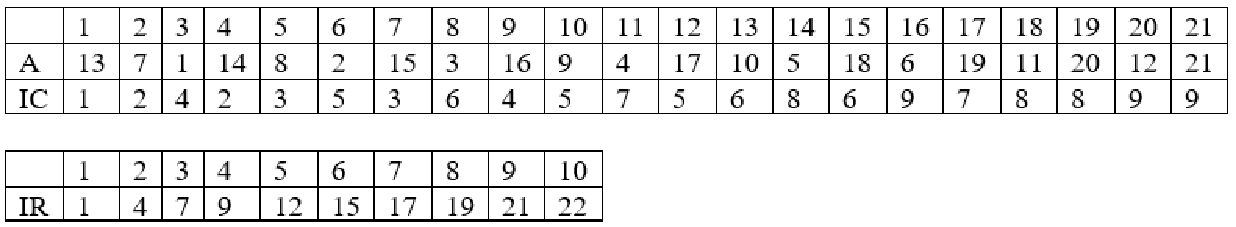
\includegraphics[width=\textwidth]{img/matrix.pdf}
  \end{figure}

  \newpage
  \subsection{Интегро-интеполяционный метод (метод баланса)}

Введем основную сетку, где N - число разбиений.
\[r_0 < r_1 < \dots < r_N,\ r_i \in [R_L, R_R],\ r_0 = R_L,\ r_N = R_R\]
\[
  h_i =r_i - r_{i-1},\ i=1,2, \dots, N
\]
\[
  r_{r-0.5} = \frac{r_i - r_{i-1}}{2},\ i=1,2, \dots, N
\]
Введем дополнительную сетку:
\[
  \hbar_i = \begin{cases}
    \frac{h_i + 1}{2},\ i = 0 \\ \\
    \frac{h_i + h_{i+1}}{2},\ i = 1, 2, \dots, N-1 \\ \\
    \frac{h_i}{2},\ i = N
  \end{cases}
\]
Проведем аппроксимацию начального уравнения.\\
Для i\ =\ 0
\[ -\int_{r_i}^{r_{i+0.5}} \left[\frac{d}{dr}\left(r k(r) \frac{du(r)}{dr}\right) -r q(r)u(r)\right]  \,dr = \int_{r_i}^{r_{i+0.5}} r f(r) \,dr, \]
\[	-\left[r k(r)\left.\frac{du(r)}{dr} \right\vert_{r=r_{i+0.5}} - r k(r) \left. \frac{du(r)}{dr}\right\vert_{r_i} - \int_{r_i}^{r_{i+0.5}} r q(r) u(r)  \,dr \right]
  = \int_{r_i}^{r_{i+0.5}} r f(r) \,dr, \]
Формула центральных разностей:
\[	\frac{du(r)}{dr}\vert_{r = r_{i+0.5}}\ \approx \frac{v_{i+1}\ -\ v_i}{h_{i+1}}, \]
Граничное условие:
\[	k(r) \left. \frac{du(r)}{dr}\right\vert_{r=R_L}\ =\ -\nu_1, \]
Формула левых прямоугольников:
\[	\int_{r_i}^{r_{r+0.5}} r \varphi_i \,dr\ =\ \hbar_i r_i \varphi_i \]
Получаем разностную схему для i = 0:
\[
  -\left[ r_{i+0.5} \cdot k_{i+0.5}\frac{v_{i+1}-v_i}{h_{i+1}} - r_i \cdot (-\nu_1) - \hbar r_i q_i v_i \right]\ =\ \hbar_ir_if_i
\]
Для i\ =\ 1, 2, \dots, N-1
\[ -\int_{r_{i-0,5}}^{r_{i+0.5}} \left[\frac{d}{dr}\left(r k(r) \frac{du(r)}{dr}\right) -r q(r)u(r)\right]  \,dr = \int_{r_{i-0.5}}^{r_{i+0.5}} r f(r) \,dr, \]
\[	-\left[r k(r)\left.\frac{du(r)}{dr} \right\vert_{r=r_{i+0.5}} - r k(r) \left. \frac{du(r)}{dr}\right\vert_{r_{i-0.5}} - \int_{r_{i-0.5}}^{r_{i+0.5}} r q(r) u(r)  \,dr \right]
= \int_{r_{i-0.5}}^{r_{i+0.5}} r f(r) \,dr, \]
\[\frac{du(r)}{dr}\vert_{r = r_{i-0.5}}\ \approx \frac{v_{i}\ -\ v_{i-1}}{h_{i}}\]
\[ \int_{r_{i-0.5}}^{r_{r+0.5}} r \varphi_i \,dr\ =\ \hbar_i r_i \varphi_i \]
Получаем разностную схему для i\ =\ 1, 2, \dots, N-1:
\[
  -\left[ r_{i+0.5} \cdot k_{i+0.5}\frac{v_{i+1}-v_i}{h_{i+1}} - r_{i-0.5}k_{i-0.5}\frac{v_{i}\ -\ v_{i-1}}{h_{i}} - \hbar r_i q_i v_i\right]\ =\ \hbar_ir_if_i
\]
Для i\ =\ N:
  \[-\int_{r_{i-0.5} }^{r_{i}} \left[\frac{d}{dr}\left(r k(r) \frac{du(r)}{dr}\right) -r q(r)u(r)\right]  \,dr = \int_{r_{i-0.5}}^{r_{i}} r f(r) \,dr, \]
  \[-\left[r k(r)\left.\frac{du(r)}{dr} \right\vert_{r=r_{i}} - r k(r) \left. \frac{du(r)}{dr}\right\vert_{r_{i-0.5}} - \int_{r_{i-0.5}}^{r_i} r q(r) u(r)  \,dr \right]
  = \int_{r_{i-0.5}}^{r_i} r f(r) \,dr, \]
  \[\frac{du(r)}{dr}\vert_{r = r_{i-0.5}}\ \approx \frac{v_{i}\ -\ v_{i-1}}{h_{i}}, \]
  \[-k(r)\left. \frac{du(r)}{dr} \right\vert_{r=R_R}\ =\ -\nu_2 \]
  \[\int_{r_{i-0.5}}^{r_i} r \varphi(r) \,dr \approx \hbar_i r_i \varphi_i \]
Получаем разностную схему для i=N:
\[
  -\left[ -r_i \cdot (-\nu_2) - r_{i-0.5}k_{i-0.5} \cdot \frac{v_i-v_{i-1}}{h_i}- \hbar_ir_iq_iu_i \right]\ =\ \hbar_ir_if_i
\]

Сгрупиируем полученные уравнения:

\[
  -\left[ r_{i+0.5} \cdot k_{i+0.5}\frac{v_{i+1}-v_i}{h_{i+1}} - r_i \cdot (-\nu_1) - \hbar r_i q_i v_i \right]\ =\ \hbar_ir_if_i \quad i = 0
\]
\[
-\left[ r_{i+0.5} \cdot k_{i+0.5}\frac{v_{i+1}-v_i}{h_{i+1}} - r_{i-0.5}k_{i-0.5}\frac{v_{i}\ -\ v_{i-1}}{h_{i}} - \hbar r_i q_i v_i\right]\ =\ \hbar_ir_if_i \quad i = 1, 2, ..., N -1
\]
\[
-\left[ -r_i \cdot (-\nu_2) - r_{i-0.5}k_{i-0.5} \cdot \frac{v_i-v_{i-1}}{h_i}- \hbar_ir_iq_iu_i \right]\ =\ \hbar_ir_if_i \quad i = N
\]

После аппроксимации уравнения можно представить в виде системы из трёхдиагональной матрицы где a, c, b - диагонали матрица A и вектора g. Элементы матрицы:\newline
Для i\ =\ 0
\begin{align*}
  c_i = r_{i+0.5}\frac{k_{i+0.5}}{h_{i+1}} + \hbar_ir_iq_i \quad
  b_i = -r_{i+0.5} \cdot \frac{k_{i+0.5}}{h_{i+1}} \quad
  g_i = \hbar_ir_if_i + r(-\nu_1)
\end{align*}
Для i\ =\ 1, 2, \dots, N-1
\begin{align*}
  a_i &= -r_{i-0.5}\frac{k_{i-0.5}}{h_i} \quad
  c_i = r_{i-0.5}\frac{k_{i-0.5}}{h_i} + r_{i+0.5}\frac{k_{i+0.5}}{h_{i+1}} + \hbar_i r_iq_i \quad
  b_i = -r_{i+0.5}\frac{k_{i+0.5}}{h_{i+1}} \\
  g_i &= \hbar_i r_i f_i
\end{align*}
Для i\ =\ N:
\begin{align*}
  a_i = -r_{i-0.5}\frac{k_{i-0.5}}{h_i} \quad
  c_i = r_{i-0.5}\frac{k_{i-0.5}}{h_i} + \hbar_i r_iq_i \quad
  g_i = \hbar_i r_i f_i + r_i \cdot (-\nu_2)
\end{align*}


  \newpage
  \section{Невязка разностной схемы}

\subsection{Невязка во внутренних точках}

Запишем для уравнения разностной сетки во внутренних точках невязку:

\begin{align*}
  &- \left [ 
  h_z r_{i+\frac{1}{2}} k_1(r_{i+\frac{1}{2}}, z_j) \frac{v_{i+1, j} - v_{i, j}}{h_{r}}
  - h_z r_{i-\frac{1}{2}} k_1(r_{i-\frac{1}{2}}, z_j) \frac{v_{i, j} - v_{i - 1, j}}{h_{r}}
  \right . \\
  &\left .
  + h_r r_{i} k_2(r_i, z_{j+\frac{1}{2}}) \frac{v_{i, j + 1} - v_{i, j}}{h_{z}}
  - h_r r_{i} k_2(r_i, z_{j-\frac{1}{2}}) \frac{v_{i, j} - v_{i, j - 1}}{h_z}
  \right ]  = h_r h_z r_i f_{i, j}
\end{align*}

\begin{align*}
  &\xi_{i, j} = h_r h_z r_i f_{i, j} + 
  \left [ 
  h_z r_{i+\frac{1}{2}} k_1(r_{i+\frac{1}{2}}, z_j) \frac{u_{i+1, j} - u_{i, j}}{h_{r}}
  - h_z r_{i-\frac{1}{2}} k_1(r_{i-\frac{1}{2}}, z_j) \frac{u_{i, j} - u_{i - 1, j}}{h_{r}}
  \right . \\
  &\left .
  + h_r r_{i} k_2(r_i, z_{j+\frac{1}{2}}) \frac{u_{i, j + 1} - u_{i, j}}{h_{z}}
  - h_r r_{i} k_2(r_i, z_{j-\frac{1}{2}}) \frac{u_{i, j} - u_{i, j - 1}}{h_z}
  \right ]
\end{align*}

Напишем разложение Тейлора для невязки:

\[
u_{i, j - 1} = u(r_i, z_j - h_z) = \left[
  u - h_z \frac{\partial u}{\partial z} + \frac{h_z^2}{2}\frac{\partial^2 u}{\partial z^2}
  - \frac{h_z^3}{6}\frac{\partial^3 u}{\partial z^3} + \frac{h_z^4}{24}\frac{\partial^4 u}{\partial z^4}
\right]_{i, j} + \mathcal{O}(h^5_y)
\]

\[
  \frac{u_{i, j} - u_{i, j - 1}}{h_z} = \left[
    \frac{\partial u}{\partial z} - \frac{h_z}{2}\frac{\partial^2 u}{\partial z^2}
    + \frac{h_z^2}{6}\frac{\partial^3 u}{\partial z^3} - \frac{h_z^3}{24}\frac{\partial^4 u}{\partial z^4}
  \right]_{i,j} + \mathcal{O}(h^4_y)
\]

\[
  r_{i} k_2(r_i, z_{j-\frac{1}{2}}) = r_i k_2(x_i, z_j - \frac{h_z}{2}) =
  \left[
   r k_2 - \frac{h_z}{2} \frac{\partial r k_2}{\partial z}
   + \frac{h_z^2}{8} \frac{\partial^2 r k_2}{\partial z^2}
   - \frac{h_z^3}{48} \frac{\partial^3 r k_2}{\partial z^3}
  \right]_{i, j} + \mathcal{O}(h^4)
\]

\begin{align*}
  r_{i} k_2(r_i, z_{j-\frac{1}{2}}) \frac{u_{i, j} - u_{i, j - 1}}{h_z} &= 
  \left[ r k_2 \frac{\partial u}{\partial z} \right]_{i, j}
  - h_z \left[
  \frac{1}{2} r k_2 \frac{\partial^2 u}{\partial z^2}
  + \frac{1}{2} \frac{\partial r k_2}{\partial z} \frac{\partial u}{\partial z}
  \right]_{i, j} +\\
  &+ h^2_z \left[
    \frac{1}{6} r k_2 \frac{\partial^3 u}{\partial z^3}
    + \frac{1}{4} \frac{\partial r k_2}{\partial z} \frac{\partial^2 u}{\partial z^2}
    + \frac{1}{8} \frac{\partial^2 r k_2}{\partial z^2} \frac{\partial u}{\partial z}
  \right]_{i, j} -\\
  &- h^3_z \left[
   \frac{1}{24} r k_2 \frac{\partial^4 u}{\partial z^4} - \frac{1}{12} \frac{\partial r k_2}{\partial z} \frac{\partial^3 u}{\partial z^3}
  + \frac{1}{16} \frac{\partial^2 r k_2}{\partial z^2} \frac{\partial^2 u}{\partial z^2}
  + \frac{1}{48} \frac{\partial^3 r k_2}{\partial z^3} \frac{\partial u}{\partial z}
   \right]_{i, j} +\\
  &+ \mathcal{O}(h^4)
\end{align*}

Для 
$
  r_{i} k_2(r_i, z_{j+\frac{1}{2}})
$
можно получить невязку аналогичным способом:

\begin{align*}
  r_{i} k_2(r_i, z_{j+\frac{1}{2}}) \frac{u_{i, j + 1} - u_{i, j}}{h_z} &= 
  \left[ r k_2 \frac{\partial u}{\partial z} \right]_{i, j}
  + h_z \left[
  \frac{1}{2} r k_2 \frac{\partial^2 u}{\partial z^2}
  + \frac{1}{2} \frac{\partial r k_2}{\partial z} \frac{\partial u}{\partial z}
  \right]_{i, j} +\\
  &+ h^2_z \left[
    \frac{1}{6} r k_2 \frac{\partial^3 u}{\partial z^3}
    + \frac{1}{4} \frac{\partial r k_2}{\partial z} \frac{\partial^2 u}{\partial z^2}
    + \frac{1}{8} \frac{\partial^2 r k_2}{\partial z^2} \frac{\partial u}{\partial z}
  \right]_{i, j} +\\
  &+ h^3_z \left[
   \frac{1}{24} r k_2 \frac{\partial^4 u}{\partial z^4} - \frac{1}{12} \frac{\partial r k_2}{\partial z} \frac{\partial^3 u}{\partial z^3}
  + \frac{1}{16} \frac{\partial^2 r k_2}{\partial z^2} \frac{\partial^2 u}{\partial z^2}
  + \frac{1}{48} \frac{\partial^3 r k_2}{\partial z^3} \frac{\partial u}{\partial z}
   \right]_{i, j} +\\
  &+ \mathcal{O}(h^4)
\end{align*}

\[
  u_{i - 1, j} = u(r_i - h_r, j) = \left[
    u - h_r \frac{\partial u}{\partial r} + \frac{h^2_r}{2}\frac{\partial^2 u}{\partial r^2}
    - \frac{h^3_r}{6}\frac{\partial^3 u}{\partial r^3} + \frac{h^4_r}{24}\frac{\partial^4 u}{\partial r^4}
  \right]_{i,j}
  + \mathcal{O}(h^5)
\]

\[
  \frac{u_{i,j} - u_{i - 1, j}}{h_r} = 
  \left[
    \frac{\partial u}{\partial r} - \frac{h_r}{2}\frac{\partial^2 u}{\partial r^2}
    + \frac{h^2_r}{6}\frac{\partial^3 u}{\partial r^3} - \frac{h^3_r}{24}\frac{\partial^4 u}{\partial r^4}
  \right]_{i,j}
  + \mathcal{O}(h^4)
\]

\[
  r_i k1 (r_{i - \frac{1}{2}}, z_j) = r_i k1(x_i - \frac{h_r}{2}, z_j) =
  \left[
  r k1 - \frac{h_r}{2}\frac{\partial rk_1}{\partial r}
  + \frac{h^2_r}{8}\frac{\partial^2 rk_1}{\partial r^2}
  - \frac{h^3_r}{48}\frac{\partial^3 rk_1}{\partial r^3}
  \right]_{i,j} + \mathcal{O}(h^4)
\]

\begin{align*}
  r_i k_1 (r_{i - \frac{1}{2}}, z_j) \frac{u_{i,j} - u_{i - 1, j}}{h_r} &= 
  \left[ rk_1 \frac{\partial u}{\partial r} \right]_{i, j} -
  h_r \left[ \frac{1}{2} rk_1 \frac{\partial^2 u}{\partial r^2} 
    + \frac{1}{2} \frac{\partial rk_1}{\partial r}\frac{\partial u}{\partial r}
  \right]_{i, j} +\\
  &+ h_r^2 \left[\frac{1}{6}rk_1\frac{\partial^3 u}{\partial r^3}
  + \frac{1}{4} \frac{\partial rk_1}{\partial r}\frac{\partial^2 u}{\partial r^2}
  + \frac{1}{8} \frac{\partial^2 rk_1}{\partial r^2}\frac{\partial u}{\partial r}
  \right]_{i, j} - \\
  &-h^3_r \left[
  \frac{1}{24} r k_1 \frac{\partial^4 u}{\partial r^4} - \frac{1}{12}\frac{\partial rk_1}{\partial r}\frac{\partial^3 u}{\partial r^3}
  + \frac{1}{16} \frac{\partial^2 rk_1}{\partial r^2}\frac{\partial^2 u}{\partial r^2}
  + \frac{1}{48} \frac{\partial^3 rk_1}{\partial r^3}\frac{\partial u}{\partial r}
  \right]_{i,j} +\\
  &+ \mathcal{O}(h^4)
\end{align*}

Для $ r_i k1(x_{i = \frac{1}{2}}, z_j) \frac{u_{i + 1, j} - u_{i, j}}{h_r} $ можно получить невязку аналогично:

\begin{align*}
  r_i k_1(x_{i + \frac{1}{2}}, z_j) \frac{u_{i + 1, j} - u_{i, j}}{h_r} &= 
  \left[ rk_1 \frac{\partial u}{\partial r} \right]_{i, j} +
  h_r \left[ \frac{1}{2} rk_1 \frac{\partial^2 u}{\partial r^2} 
    + \frac{1}{2} \frac{\partial rk_1}{\partial r}\frac{\partial u}{\partial r}
  \right]_{i, j} +\\
  &+ h_r^2 \left[\frac{1}{6}rk_1\frac{\partial^3 u}{\partial r^3}
  + \frac{1}{4} \frac{\partial rk_1}{\partial r}\frac{\partial^2 u}{\partial r^2}
  + \frac{1}{8} \frac{\partial^2 rk_1}{\partial r^2}\frac{\partial u}{\partial r}
  \right]_{i, j} + \\
  &+ h^3_r \left[
  \frac{1}{24} r k_1 \frac{\partial^4 u}{\partial r^4} - \frac{1}{12}\frac{\partial rk_1}{\partial r}\frac{\partial^3 u}{\partial r^3}
  + \frac{1}{16} \frac{\partial^2 rk_1}{\partial r^2}\frac{\partial^2 u}{\partial r^2}
  + \frac{1}{48} \frac{\partial^3 rk_1}{\partial r^3}\frac{\partial u}{\partial r}
  \right]_{i,j} +\\
  &+ \mathcal{O}(h^4)
\end{align*}

Тогда:

\begin{align*}
  &r_i k_1(x_{i + \frac{1}{2}}, z_j) \frac{u_{i + 1, j} - u_{i, j}}{h_r} - r_i k_1 (r_{i - \frac{1}{2}}, z_j) \frac{u_{i,j} - u_{i - 1, j}}{h_r} =
  h_r h_z \left( \left[ rk_1 \frac{\partial^2 u}{\partial r^2} + \frac{\partial rk_1}{\partial r}\frac{\partial u}{\partial r} \right]_{i, j} \right. + \\
  &+ \left. h^2_r\left[ \frac{1}{12} r k_1 \frac{\partial^4 u}{\partial r^4} - \frac{1}{6}\frac{\partial rk_1}{\partial r}\frac{\partial^3 u}{\partial r^3}
  + \frac{1}{8} \frac{\partial^2 rk_1}{\partial r^2}\frac{\partial^2 u}{\partial r^2}
  + \frac{1}{24} \frac{\partial^3 rk_1}{\partial r^3}\frac{\partial u}{\partial r} \right] + \mathcal{O}(h_r^4) \right)
\end{align*}


\begin{align*}
  &r_{i} k_2(r_i, z_{j+\frac{1}{2}}) \frac{u_{i, j + 1} - u_{i, j}}{h_z} - r_{i} k_2(r_i, z_{j-\frac{1}{2}}) \frac{u_{i, j} - u_{i, j - 1}}{h_z} =
  h_r h_z \left(
    \left[ r k_2 \frac{\partial^2 u}{\partial z^2}
    + \frac{\partial r k_2}{\partial z} \frac{\partial u}{\partial z} \right]_{i, j}
   \right. +\\
  &+ \left. h^2_z \left[
    \frac{1}{12} r k_2 \frac{\partial^4 u}{\partial z^4} - \frac{1}{6} \frac{\partial r k_2}{\partial z} \frac{\partial^3 u}{\partial z^3}
    + \frac{1}{8} \frac{\partial^2 r k_2}{\partial z^2} \frac{\partial^2 u}{\partial z^2}
    + \frac{1}{24} \frac{\partial^3 r k_2}{\partial z^3} \frac{\partial u}{\partial z}
     \right]_{i, j} + \mathcal{O}(h_z^4) \right)
\end{align*}

Будем искать невязку в следующем виде:
\[
  \tilde{\xi}_{i, j} = \frac{\xi_{i, j}}{h_r h_z}
\]

Тогда:
\begin{align*}
  &\tilde{\xi}_{i, j} = r_if_{i, j} + \left[ rk_1 \frac{\partial^2 u}{\partial r^2} + \frac{\partial rk_1}{\partial r}\frac{\partial u}{\partial r} \right]_{i, j} \left[ r k_2 \frac{\partial^2 u}{\partial z^2}
  + \frac{\partial r k_2}{\partial z} \frac{\partial u}{\partial z} \right]_{i, j} + \\
  &+h^2_r\left[ \frac{1}{12} r k_1 \frac{\partial^4 u}{\partial r^4} - \frac{1}{6}\frac{\partial rk_1}{\partial r}\frac{\partial^3 u}{\partial r^3}
  + \frac{1}{8} \frac{\partial^2 rk_1}{\partial r^2}\frac{\partial^2 u}{\partial r^2}
  + \frac{1}{24} \frac{\partial^3 rk_1}{\partial r^3}\frac{\partial u}{\partial r} \right] + \mathcal{O}(h_r^3) + \\
  &+ h^2_z \left[
    \frac{1}{12} r k_2 \frac{\partial^4 u}{\partial z^4} - \frac{1}{6} \frac{\partial r k_2}{\partial z} \frac{\partial^3 u}{\partial z^3}
    + \frac{1}{8} \frac{\partial^2 r k_2}{\partial z^2} \frac{\partial^2 u}{\partial z^2}
    + \frac{1}{24} \frac{\partial^3 r k_2}{\partial z^3} \frac{\partial u}{\partial z}
     \right]_{i, j} + \mathcal{O}(h_z^3)
\end{align*}

Можно заметить, что:
\[
  \left[ rk_1 \frac{\partial^2 u}{\partial r^2} + \frac{\partial rk_1}{\partial r}\frac{\partial u}{\partial r} \right]_{i, j} =
  \frac{\partial}{\partial r} \left( k_1 \frac{\partial u}{\partial r} \right)
\]

\[
  \left[ r k_2 \frac{\partial^2 u}{\partial z^2} + \frac{\partial r k_2}{\partial z} \frac{\partial u}{\partial z} \right]_{i, j} =
  \frac{\partial}{\partial z} \left( k_2 \frac{\partial u}{\partial z} \right)
\]

Тем самым:
\[
  r_if_{i, j} + \frac{\partial}{\partial r} \left( k_1 \frac{\partial u}{\partial r} \right) +
  \frac{\partial}{\partial z} \left( k_2 \frac{\partial u}{\partial z} \right) = 0
\]

Получаем:
\begin{align*}
  &\tilde{\xi}_{i, j} = 
  h^2_r\left[ \frac{1}{12} r k_1 \frac{\partial^4 u}{\partial r^4} - \frac{1}{6}\frac{\partial rk_1}{\partial r}\frac{\partial^3 u}{\partial r^3}
  + \frac{1}{8} \frac{\partial^2 rk_1}{\partial r^2}\frac{\partial^2 u}{\partial r^2}
  + \frac{1}{24} \frac{\partial^3 rk_1}{\partial r^3}\frac{\partial u}{\partial r} \right] + \mathcal{O}(h_r^3) + \\
  &+ h^2_z \left[
    \frac{1}{12} r k_2 \frac{\partial^4 u}{\partial z^4} - \frac{1}{6} \frac{\partial r k_2}{\partial z} \frac{\partial^3 u}{\partial z^3}
    + \frac{1}{8} \frac{\partial^2 r k_2}{\partial z^2} \frac{\partial^2 u}{\partial z^2}
    + \frac{1}{24} \frac{\partial^3 r k_2}{\partial z^3} \frac{\partial u}{\partial z}
     \right]_{i, j} + \mathcal{O}(h_z^3)
\end{align*}

Порядок апроксимации $p_r = 2 - 0 $, $ p_z = 2 - 0 $.

\subsection{Невязка на левой границе}

  \newpage
  \section{Запись СЛАУ}

Перейдём к одноиндексной записи

\[
  m = j(N_r + 1) + i
\]

Индексы изменяются в следующих границах:
\[
  0 \leq i \leq N_r
\]

\[
  0 \leq j \leq N_z
\]

Тогда имеем:
\[
  0 \leq m < (N_r + 1)(N_y + 1)
\]

\subsection{Запись для внутренних точек}
Перепишем наше уравнение с использованием нового индеса для $ i \in (0, N_r)$ и $ j \in (0, N_z) $:

\begin{align*}
  &- \left [ 
  h_z r_{i+\frac{1}{2}} k_1(r_{i+\frac{1}{2}}, z_j) \frac{v_{i+1, j} - v_{i, j}}{h_{r}}
  - h_z r_{i-\frac{1}{2}} k_1(r_{i-\frac{1}{2}}, z_j) \frac{v_{i, j} - v_{i - 1, j}}{h_{r}}
  \right . \\
  &\left .
  + h_r r_{i} k_2(r_i, z_{j+\frac{1}{2}}) \frac{v_{i, j + 1} - v_{i, j}}{h_{z}}
  - h_r r_{i} k_2(r_i, z_{j-\frac{1}{2}}) \frac{v_{i, j} - v_{i, j - 1}}{h_z}
  \right ]  = h_r h_z r_i f_{i, j}
\end{align*}

\begin{align*}
  & -\frac{h_r}{h_z} r_i k_2(r_i, z_{j - \frac{1}{2}}) v_{i, j - 1} - \frac{h_z}{h_r} r_{i - \frac{1}{2}} k_1(r_{i - \frac{1}{2}}, z_j) v_{i - 1, j} + \\
  & + \left[ 
    \frac{h_z}{h_r} r_{i + \frac{1}{2}} k_1(r_{i + \frac{1}{2}}, z_j) + \frac{h_z}{h_r} r_{i - \frac{1}{2}} k_1(r_{i - \frac{1}{2}}, z_j) +
    \frac{h_r}{h_z} r_i k_2 (r_i, z_{j + \frac{1}{2}}) + \frac{h_r}{h_z} r_i k_2 (r_i, z_{j-\frac{1}{2}})
   \right] v_{i, j} \\
  & - \frac{h_z}{h_r} r_{i + \frac{1}{2}} k_1(r_{i+ \frac{1}{2}}, z_j) v_{i + 1, j} - \frac{h_r}{h_z} r_i k_2(r_i, z_{j + 1}) v_{i, j + \frac{1}{2}}
  = h_r h_z r_i f_{i, j}
\end{align*}

Введём новые обозначения:

\[
  a_m w_{m - L} + b_m w_{m - 1} + c_m w_m + d_m w_{m + 1} + e_m w_{m + L} = g_m
\]

где коэффициенты равны:
\[
  a_m = -\frac{h_r}{h_z} r_i k_2(r_i, z_{j - \frac{1}{2}})
\]

\[
  b_m = - \frac{h_z}{h_r} r_{i - \frac{1}{2}} k_1(r_{i - \frac{1}{2}}, z_j)
\]

\[
  c_m = \frac{h_z}{h_r} r_{i + \frac{1}{2}} k_1(r_{i + \frac{1}{2}}, z_j) + \frac{h_z}{h_r} r_{i - \frac{1}{2}} k_1(r_{i - \frac{1}{2}}, z_j) +
  \frac{h_r}{h_z} r_i k_2 (r_i, z_{j + \frac{1}{2}}) + \frac{h_r}{h_z} r_i k_2 (r_i, z_{j-\frac{1}{2}})
\]

\[
  d_m = - \frac{h_z}{h_r} r_{i + \frac{1}{2}} k_1(r_{i+ \frac{1}{2}}, z_j)
\]

\[
  e_m = - \frac{h_r}{h_z} r_i k_2(r_i, z_{j + 1})
\]

\[
  g_m = h_r h_z r_i f_{i, j}
\]

\subsection{Запись для левой границы}

Перепишем наше уравнение с использованием нового индекса для $i = 0$ и $ j \in (0, N_z) $:

\begin{align*}
  &- \left [ 
    h_z r_{\frac{1}{2}} k_1(r_{\frac{1}{2}}, z_j) \frac{v_{1, j} - v_{0, j}}{h_{r}}
    - 0
    \right . \\
    &\left .
    + \frac{h_r}{2} \frac{r_{\frac{1}{2}}}{2} k_2(r_0, z_{j+\frac{1}{2}}) \frac{v_{0, j + 1} - v_{0, j}}{h_{z}}
    - \frac{h_r}{2} \frac{r_{\frac{1}{2}}}{2} k_2(r_0, z_{j-\frac{1}{2}}) \frac{v_{0, j} - v_{0, j - 1}}{h_z}
    \right ]  = \frac{h_r}{2} \frac{r_{\frac{1}{2}}}{2} h_z f_{0, j}
\end{align*}

\begin{align*}
  & - \frac{h_r}{2 h_z} \frac{r_{\frac{1}{2}}}{2} k_2(r_0, z_{j - \frac{1}{2}}) v_{0, j - 1} + \\
  & + \left[
    \frac{h_z}{h_r} r_{\frac{1}{2}} k_1(r_{\frac{1}{2}}, z_j) + \frac{h_r}{2 h_z} \frac{r_{\frac{1}{2}}}{2} k_2(r_0, z_{j+\frac{1}{2}})
    + \frac{h_r}{2 h_z} \frac{r_{\frac{1}{2}}}{2} k_2(r_0, z_{j -\frac{1}{2}})
  \right] v_{0, j} \\
  & - \frac{h_z}{h_r} r_{\frac{1}{2}} k_1(r_{\frac{1}{2}}, z_j) v_{1, j}
  - \frac{h_r}{2 h_z} \frac{r_{\frac{1}{2}}}{2} k_2(r_0, z_{j + \frac{1}{2}}) v_{0, j + 1} = \frac{h_r}{2} \frac{r_{\frac{1}{2}}}{2} h_z f_{0, j}
\end{align*}

Введём новые обозначения:

\[
  a_m w_{m - L} + c_m w_m + d_m w_{m + 1} + e_m w_{m + L} = g_m
\]

где коэффициенты равны:

\[
  a_m = - \frac{h_r}{2 h_z} \frac{r_{\frac{1}{2}}}{2} k_2(r_0, z_{j - \frac{1}{2}})
\]

\[
  c_m = \frac{h_z}{h_r} r_{\frac{1}{2}} k_1(r_{\frac{1}{2}}, z_j) + \frac{h_r}{2 h_z} \frac{r_{\frac{1}{2}}}{2} k_2(r_0, z_{j+\frac{1}{2}})
  + \frac{h_r}{2 h_z} \frac{r_{\frac{1}{2}}}{2} k_2(r_0, z_{j -\frac{1}{2}})
\]

\[
  d_m = - \frac{h_z}{h_r} r_{\frac{1}{2}} k_1(r_{\frac{1}{2}}, z_j)
\]

\[
  e_m = - \frac{h_r}{2 h_z} \frac{r_{\frac{1}{2}}}{2} k_2(r_0, z_{j + \frac{1}{2}})
\]

\[
  g_m = \frac{h_r}{2} \frac{r_{\frac{1}{2}}}{2} h_z f_{0, j}
\]

\subsection{Запись для правой границы}
Перепишем наше уравнение с использованием нового индекса для $i = N_r$ и $ j \in (0, N_z) $:

\begin{align*}
  &- \left [ 
  -h_z ( \chi_2 v_{N_r} - \varphi_2(z))
  - h_z r_{N_r-\frac{1}{2}} k_1(r_{N_r-\frac{1}{2}}, z_j) \frac{v_{N_r, j} - v_{N_r - 1, j}}{h_{r}}
  \right . \\
  &\left .
  + \frac{h_r}{2} r_{N_r} k_2(r_{N_r}, z_{j+\frac{1}{2}}) \frac{v_{N_r, j + 1} - v_{N_r, j}}{h_{z}}
  - \frac{h_r}{2} r_{N_r} k_2(r_{N_r}, z_{j-\frac{1}{2}}) \frac{v_{N_r, j} - v_{N_r, j - 1}}{h_z}
  \right ]  = \frac{h_r}{2} r_{N_r} h_z f_{N_r, j}
\end{align*}

\begin{align*}
  & - \frac{h_r}{2h_z} r_{N_r} k_2(r_{N_r}, z_{j - \frac{1}{2}}) v_{N_r, j - 1}
  - \frac{h_z}{h_r} r_{N_r - \frac{1}{2}} k_1(r_{N_r - \frac{1}{2}}, z_j) v_{N_r - 1, j} \\
  & +\left[
    h_z\chi_2  + \frac{h_z}{h_r} r_{N_r - \frac{1}{2}} k_1(r_{N_r -\frac{1}{2}}, z_j)
    + \frac{h_r}{2 h_z} r_{N_r} k_2(r_{N_r, z_{j + \frac{1}{2}}})
    + \frac{h_r}{2 h_z} r_{N_r} k_2 (r_{N_r}, z_{j - \frac{1}{2}})
  \right] v_{N_r, j} \\
  &- \frac{h_r}{2 h_z} r_{N_r} k_2(r_{N_r}, z_{j + \frac{1}{2}}) v_{N_r, j + 1}
  = \frac{h_r}{2} r_{N_r} h_z f_{N_r, j} + h_z\phi_2(z)
\end{align*}

Введём новые обозначения:
\[
  a_m w_{m - L} + b_m w_{m - 1} + c_m w_m + e_m w_{m + L} = g_m
\]

где коэффициенты:

\[
  a_m = - \frac{h_r}{2h_z} r_{N_r} k_2(r_{N_r}, z_{j - \frac{1}{2}})
\]

\[
  b_m = - \frac{h_z}{h_r} r_{N_r - \frac{1}{2}} k_1(r_{N_r - \frac{1}{2}}, z_j)
\]

\[
  c_m = h_z\chi_2  + \frac{h_z}{h_r} r_{N_r - \frac{1}{2}} k_1(r_{N_r -\frac{1}{2}}, z_j)
  + \frac{h_r}{2 h_z} r_{N_r} k_2(r_{N_r, z_{j + \frac{1}{2}}})
  + \frac{h_r}{2 h_z} r_{N_r} k_2 (r_{N_r}, z_{j - \frac{1}{2}})
\]

\[
  e_m = - \frac{h_r}{2 h_z} r_{N_r} k_2(r_{N_r}, z_{j + \frac{1}{2}})
\]

\[
  g_m =\frac{h_r}{2} r_{N_r} h_z f_{N_r, j} + h_z\varphi_2(z)
\]

\subsection{Запись для нижней границы}
Перепишем наше уравнение с использованием нового индекса для $i \in (0, N_r) $ и $ j = 0 $:

\begin{align*}
  - \left [ 
  \frac{h_z}{2} r_{i+\frac{1}{2}} k_1(r_{i+\frac{1}{2}}, z_0) \frac{v_{i+1, 0} - v_{i, 0}}{h_{r}}
  - \frac{h_z}{2} r_{i-\frac{1}{2}} k_1(r_{i-\frac{1}{2}}, z_0) \frac{v_{i, 0} - v_{i - 1, 0}}{h_{r}}
  \right . \\
  \left .
  + h_r r_{i} k_2(r_i, z_{\frac{1}{2}}) \frac{v_{i, 1} - v_{i, 0}}{h_{z}}
  - h_r(\chi_3 v_{i, 0} - \varphi_3(r))
  \right ]  = h_r \frac{h_z}{2} r_i f_{i, 0}
\end{align*}

\begin{align*}
  &  - \frac{h_z}{2 h_r} v_{i - \frac{1}{2}} k_1(r_{i - \frac{1}{2}}, z_0) v_{i - 1, 0} \\
  & + \left[ 
    h_r \chi_3 +\frac{h_z}{2 h_r} r_{i + \frac{1}{2}} k_1(r_{i + \frac{1}{2}}, z_0) + \frac{h_z}{2 h_r} r_{i - \frac{1}{2}} k_1(r_{i - \frac{1}{2}}, z_0)
    + \frac{h_r}{h_z} r_i k_2(r_i, z_{\frac{1}{2}}) 
  \right] v_{i, 0} \\
  & - \frac{h_z}{2 h_r} r_{i + \frac{1}{2}} k_1(r_{i + \frac{1}{2}}, z_0) v_{i + 1, 0} - \frac{h_r}{h_z} r_i k_2 (r_i, z_{\frac{1}{2}}) v_{i, 1}
  = h_r \frac{h_z}{2} r_i f_{i, 0} + h_r \varphi(r)
\end{align*}

Введём новые обозначения:
\[
  b_m w_{m - 1} + c_m w_m + d_m w_{m + 1} + e_m w_{m + L} = g_m
\]

где коэффициенты ранвы:
\[
  b_m = - \frac{h_z}{2 h_r} r_{i - \frac{1}{2}} k_1(r_{i - \frac{1}{2}}, z_0)
\]

\[
  c_m = h_r \chi_3 +\frac{h_z}{2 h_r} r_{i + \frac{1}{2}} k_1(r_{i + \frac{1}{2}}, z_0) + \frac{h_z}{2 h_r} r_{i - \frac{1}{2}} k_1(r_{i - \frac{1}{2}}, z_0)
  + \frac{h_r}{h_z} r_i k_2(r_i, z_{\frac{1}{2}}) 
\]

\[
  d_m = - \frac{h_z}{2 h_r} r_{i + \frac{1}{2}} k_1(r_{i + \frac{1}{2}}, z_0)
\]

\[
  e_m = - \frac{h_r}{h_z} r_i k_2 (r_i, z_{\frac{1}{2}})
\]

\[
  g_m = h_r \frac{h_z}{2} r_i f_{i, 0} + h_r \varphi_3(r)
\]

\subsection{Запись для верхней границы}
Перепишем наше уравнение с использованием нового индекса для $i \in [0, N_r] $ и $ j = N_z $:

\[
  v_{i, N_z} = \varphi(r_i)
\]

Перейдём к новым обозначениям:
\[
  c_m w_m = \varphi_m
\]

где:
\[
  c_m = 1, \quad \varphi_m = \varphi_2(r_i)
\]


\subsection{Запись для левой нижней граничной точки}

Перепишем наше уравнение с использованием нового индекса для $i = 0 $ и $ j = 0 $:

\begin{align*}
  &- \left [ 
  \frac{h_z}{2} r_{\frac{1}{2}} k_1(r_{\frac{1}{2}}, z_0) \frac{v_{1, 0} - v_{0, 0}}{h_{r}}
  - 0
  \right . \\
  &\left .
  + \frac{h_r}{2} \frac{r_{\frac{1}{2}}}{2} k_2(r_0, z_{\frac{1}{2}}) \frac{v_{0, 1} - v_{0, 0}}{h_{z}}
  - \frac{h_r}{2} \frac{r_{\frac{1}{2}}}{2} (\chi_3 v_{0, 0} - \varphi_3(r))
  \right ]  = \frac{h_r}{2} \frac{h_z}{2} \frac{r_{\frac{1}{2}}}{2} f_{0, 0}
\end{align*}

\begin{align*}
  &\left[
    \frac{h_z}{2 h_r} r_{\frac{1}{2}} k_1(r_{\frac{1}{2}}, z_0) + \frac{h_r}{2 h_z} \frac{r_{\frac{1}{2}}}{2} k_2(r_0, z_{\frac{1}{2}}) + \frac{h_r}{2} \chi_3
  \right] v_{0, 0} - \\
  & - \frac{h_z}{2 h_r} r_\frac{1}{2} k_1(r_\frac{1}{2}, z_0) v_{1,0} 
  - \frac{h_r}{2 h_z} \frac{r_{\frac{1}{2}}}{2} k_2(r_0, z_{\frac{1}{2}}) v_{0, 1}
  = \frac{h_r}{2} \frac{h_z}{2} \frac{r_{\frac{1}{2}}}{2} f_{0, 0} + \frac{h_r}{2} \frac{r_{\frac{1}{2}}}{2} \varphi_3(r_0)
\end{align*}

Введём новые обозначения:
\[
  c_m w_m + d_m w_{m + 1} + e_m w_{m + L} = g_m
\]

где коэффициенты ранвы:

\[
  c_m = \frac{h_z}{2 h_r} r_{\frac{1}{2}} k_1(r_{\frac{1}{2}}, z_0) + \frac{h_r}{2 h_z} \frac{r_{\frac{1}{2}}}{2} k_2(r_0, z_{\frac{1}{2}}) + \frac{h_r}{2} \chi_3
\]

\[
  d_m = - \frac{h_z}{2 h_r} r_\frac{1}{2} k_1(r_\frac{1}{2}, z_0)
\]

\[
  e_m = - \frac{h_r}{2 h_z} \frac{r_{\frac{1}{2}}}{2} k_2(r_0, z_{\frac{1}{2}})
\]

\[
  g_m = \frac{h_r}{2} \frac{h_z}{2} \frac{r_{\frac{1}{2}}}{2} f_{0, 0} + \frac{h_r}{2} \frac{r_{\frac{1}{2}}}{2} \varphi_3(r_0)
\]

\subsection{Запись для правой нижней граничной точки}

Перепишем наше уравнение с использованием нового индекса для $i = N_r $ и $ j = 0 $:

\begin{align*}
  - \left [ 
  -\frac{h_z}{2} (\chi_2 v_{N_r, 0} - \varphi_2(z) )
  - \frac{h_z}{2} r_{N_r-\frac{1}{2}} k_1(r_{N_r-\frac{1}{2}}, z_0) \frac{v_{N_r, 0} - v_{N_r - 1, 0}}{h_{r}}
  \right . \\
  \left .
  + \frac{h_r}{2} r_{N_r} k_2(r_{N_r}, z_{\frac{1}{2}}) \frac{v_{N_r, 1} - v_{N_r, 0}}{h_{z}}
  - \frac{h_r}{2}(\chi_3 v_{N_r, 0} - \varphi_3(r))
  \right ]  = \frac{h_r}{2} \frac{h_z}{2} r_{N_r} f_{N_r, 0}
\end{align*}

\begin{align*}
  & - \frac{h_z}{2 h_r} r_{N_r - \frac{1}{2}} k_1 (r_{N_r - \frac{1}{2}}, z_0) v_{N_r - 1, 0} +\\
  & + \left[
    \frac{h_z}{2} \chi_2 + \frac{h_z}{2 h_r} r_{N_r - \frac{1}{2}} k_1 (r_{N_r - \frac{1}{2}}, z_0) 
    + \frac{h_r}{2 h_z} r_{N_r} k_2(r_{N_r, z_{\frac{1}{2}}}) + \frac{h_r}{2} \chi_3
  \right] v_{N_r, 0} - \\
  & - \frac{h_r}{2 h_z} r_{N_r} k_2(r_{N_r}, z_{\frac{1}{2}}) v_{N_r, 1}
  = \frac{h_r}{2} \frac{h_z}{2} r_{N_r} f_{N_r, 0} + \frac{h_z}{2} \varphi_2(z) + \frac{h_r}{2} \varphi_3(r)
\end{align*}

Введём новые обозначения:
\[
  b_m w_{m - 1} + c_m w_m + e_m w_{m + L} = g_m
\]

где коэффициенты равны:

\[
  b_m = - \frac{h_z}{2 h_r} r_{N_r - \frac{1}{2}} k_1 (r_{N_r - \frac{1}{2}}, z_0)
\]

\[
  c_m = \frac{h_z}{2} \chi_2 + \frac{h_z}{2 h_r} r_{N_r - \frac{1}{2}} k_1 (r_{N_r - \frac{1}{2}}, z_0) 
  + \frac{h_r}{2 h_z} r_{N_r} k_2(r_{N_r, z_{\frac{1}{2}}}) + \frac{h_r}{2} \chi_3
\]

\[
  e_m = - \frac{h_r}{2 h_z} r_{N_r} k_2(r_{N_r}, z_{\frac{1}{2}}) 
\]

\[
  g_m = \frac{h_r}{2} \frac{h_z}{2} r_{N_r} f_{N_r, 0} + \frac{h_z}{2} \varphi_2(z) + \frac{h_r}{2} \varphi_3(r)
\]

  \newpage
  \section{Метод сопряжённых градиентов}

Для решения системы линейных алгебраических уравнений использовать метод
сопряженных градиентов с предобусловливанием. Опишем метод решения следующей системы:

\[
  Ax = b
\]

где A - симметричная, положительно определённая, матрица.

\subsection{Явный метод}

\RestyleAlgo{tworuled}
\SetAlFnt{\normalsize}
\SetAlgoNoLine

\begin{algorithm*}[H]
  \DontPrintSemicolon
  $r^{(0)} = b - Ax^{(0)} $ \;
  $s^{(1)} = r^{(0)} $ \;
  $ \gamma = \sqrt{(b, b)} $

  \For{$k = 1$ \KwTo $k_{max}$}{
    $\displaystyle
        \alpha_k = \frac{\left( r^{(k-1)},\ r^{(k-1)} \right)}{\left( As^{(k)},\ s^{(k)} \right)}
    $\;
    $x^{(k)} = x^{(k-1)} + \alpha_k s^{(k)}$\;
    $r^{(k)} = r^{(k-1)} - \alpha_k s^{(k-1)}$\;

    \If{$\sqrt{\left( r^{(k)},\ r^{(k)} \right)} < \gamma \varepsilon $}{
        \textbf{break}
    }

    $\displaystyle
        \beta_k = \frac{\left( r^{(k)},\ r^{(k)} \right)}{\left( r^{(k-1)},\ r^{(k-1)} \right)}
    $\;
    $s^{(k+1)} = r^{(k)} + \beta_k s^{(k)}$\;
}
\end{algorithm*}

\subsection{Неявный метод}

еявный метод основывается на использовании предобуславливания. 
Идея заключается в том, чтобы выбрать матрицу \textbf{B}, которая является
симметричной и положительно определенной, и приблизительно равна 
матрице \textbf{A}. Мы выбираем \textbf{B} в виде
$B = \Tilde{L} \Tilde{L}^T $, где $\Tilde{L} \Tilde{L}^T$ представляет собой 
неполное разложение Холецкого для матрицы \textbf{A}.
Позже мы объясним, почему такой выбор матрицы \textbf{B} считается оптимальным.

\begin{algorithm*}[H]
  
  \DontPrintSemicolon

  $r^{(0)} = b - A x^{(0)}$\;
  $B w^{(0)} = r^{(0)}$\;
  $s^{(1)} = w^{(0)}$\;
  $B g = b$\;
  $\gamma = \sqrt{\left( g,\ b \right)}$\;

  \For{$k = 1$ \KwTo $k_{max}$}{
      $\displaystyle
          \alpha_k = \frac{\left( w^{(k-1)},\ r^{(k-1)} \right)}{\left( As^{(k)},\ s^{(k)} \right)}
      $\;
      $x^{(k)} = x^{(k-1)} + \alpha_k s^{(k)}$\;
      $r^{(k)} = r^{(k-1)} - \alpha_k s^{(k-1)}$\;
      $Bw^{(k)} = r^{(k)}$\;

      \If{$\sqrt{\left( w^{(k)},\ r^{(k)} \right)} < \gamma \varepsilon $}{
          \textbf{break}
      }

      $\displaystyle
          \beta_k = \frac{\left( w^{(k)},\ r^{(k)} \right)}{\left( w^{(k-1)},\ r^{(k-1)} \right)}
      $\;
      $s^{(k+1)} = w^{(k)} + \beta_k s^{(k)}$\;
  }
\end{algorithm*}

Для решения системы $Bw(k) = r(k)$ мы используем метод Гаусса.
При выборе $B = \Tilde{L} \Tilde{L}^T $, нам остается выполнить только две обратные подстановки:
$ \Tilde{L} z^{(k)} = r^{k} $ и $ \Tilde{L}^T w^{(k)} = z^{(k)}$.

  \newpage
  \section{Тестирование}

Протестируем постренную модель на следующих тестовых наборах:

\begin{center}
  \begin{tabular}{*4{c}}
  \toprule
  \makecell{№ \\ теста} & $k_1(r, z)$ & $k_2(r, z)$ & $ u(r, z)$ \\
  \midrule
  1 & $ r + z + 3 $ & $ r + z + 3 $ & $1$ \\
  2 & $ 3r + 2z + 1 $ & $ 3r + 2z + 1 $ & $r^2$ \\
  3 & $ (r + z + 3)^2 $ & $ (r + z + 3)^2 $ & $(r + 2z)^2$ \\
  4 & $ (r + 2z + 3)^3 $ & $ (r + 2z + 3)^3 $ & $r^3 + z^2$ \\
  \bottomrule
  \end{tabular}
\end{center}

Все тесты имеют общие значения:

\[
  r \in [0, 1],\quad z \in [0, 2]
\]

\[
  \chi_2 = 2,\quad \chi_3 = 3
\]

Функция $f$, $ \varphi_2 $, $ \varphi_3 $, $\varphi_4$ вычисляют программно
с использованием символичных вычислений и не приведены в описании тестов.

Погрешность решения задачи вычисляется следующим образом:
\[
\delta_1 = \frac{\left|| v - \Tilde{v} \right||_1 }{\left|| v \right||_1 }
\]

\[
\delta_2 = \frac{\left|| v - \Tilde{v} \right||_2 }{\left|| v \right||_2 }
\]

\[
\delta_3 = \frac{\left|| v - \Tilde{v} \right||_\infty }{\left|| v \right||_\infty }
\]

Значение $ \varepsilon $ для метода сопряжённых градиентов равно $ 10^{-8} $.

\subsubsection*{Тест №1}

Имеем лишь ошибку округления.

\begin{table}[H]
\begin{center}
  \begin{tabular}{*{6}c}
    \toprule
    $ N_r $ & $ N_z $ & n & $ \delta_1 $ & $ \delta_2 $ & $ \delta_3 $ \\
    \midrule
    2 & 2 & 8 & $4.324e-16 $ & $7.63e-16 $ & $4.064e-16 $ \\
    4 & 4 & 27 & $2.514e-11 $ & $2.419e-11 $ & $2.88e-11 $ \\
    8 & 8 & 62 & $1.354e-10 $ & $1.284e-10 $ & $1.868e-10 $ \\
    16 & 16 & 117 & $2.3e-10 $ & $6.527e-10 $ & $1.151e-10 $ \\
    32 & 32 & 306 & $5.921e-09 $ & $1.849e-09 $ & $4.102e-09 $ \\
    \bottomrule
  \end{tabular}
  \caption{Явный метод}
\end{center}
\end{table}

\begin{table}[H]
  \begin{center}
    \begin{tabular}{*{6}c}
      \toprule
      $ N_r $ & $ N_z $ & n & $ \delta_1 $ & $ \delta_2 $ & $ \delta_3 $ \\
      \midrule
      2 & 2 & 5 & $ 9.509e-16 $ & $ 4.186e-16 $ & $ 9.29e-16 $ \\
      4 & 4 & 9 & $2.395e-11 $ & $2.574e-11 $ & $4.137e-11 $ \\
      8 & 8 & 15 & $ 1.62e-10 $ & $2.34e-10 $ & $1.97e-10 $ \\
      16 & 16 & 25 & $6.74e-10$ & $9.82e-10 $ & $2.23e-10 $ \\
      32 & 32 & 46 & $1.12e-9 $ & $1.59e-9 $ & $3.37e-9 $ \\
      \bottomrule
    \end{tabular}
    \caption{Неявный метод}
  \end{center}
\end{table}

\subsubsection*{Тест №2}

Присутствует ошибка округления и ошибка аппроксимации.

\begin{table}[H]
  \begin{center}
    \begin{tabular}{*{6}c}
      \toprule
      $ N_r $ & $ N_z $ & n & $ \delta_1 $ & $ \delta_2 $ & $ \delta_3 $ \\
      \midrule
      2 & 2 & 8 & $3.471e-4 $ & $4.164e-4 $ & $7.953e-4 $ \\
      4 & 4 & 21 & $8.689e-5 $ & $1.041e-4 $ & $1.986e-4 $ \\
      8 & 8 & 55 & $2.181e-5 $ & $2.624e-5 $ & $4.971e-5 $ \\
      16 & 16 & 107 & $5.378e-6 $ & $6.47e-6 $ & $1.249e-5 $ \\
      32 & 32 & 208 & $1.485e-6 $ & $1.589e-6 $ & $3.136e-6 $ \\
      \bottomrule
    \end{tabular}
    \caption{Явный метод}
  \end{center}
  \end{table}
  
  \begin{table}[H]
    \begin{center}
      \begin{tabular}{*{6}c}
        \toprule
        $ N_r $ & $ N_z $ & n & $ \delta_1 $ & $ \delta_2 $ & $ \delta_3 $ \\
        \midrule
        2 & 2 & 5 & $3.471e-4 $ & $4.164e-4 $ & $7.953e-4 $  \\
        4 & 4 & 8 & $8.689e-5 $ & $1.041e-4 $ & $1.986e-4 $ \\
        8 & 8 & 14 & $2.181e-5 $ & $2.624e-5 $ & $4.971e-5 $ \\
        16 & 16 & 27 & $5.378e-6 $ & $6.47e-6 $ & $1.249e-5 $ \\
        32 & 32 & 44 & $1.485e-6 $ & $1.589e-6 $ & $3.136e-6 $ \\
        \bottomrule
      \end{tabular}
      \caption{Неявный метод}
    \end{center}
  \end{table}

\subsubsection*{Тест №3}

Присутствует ошибка округления и ошибка аппроксимации.

\begin{table}[H]
  \begin{center}
    \begin{tabular}{*{6}c}
      \toprule
      $ N_r $ & $ N_z $ & n & $ \delta_1 $ & $ \delta_2 $ & $ \delta_3 $ \\
      \midrule
      2 & 2 & 7 & $6.74e-2 $ & $7.374e-2 $ & $6.27e-2 $ \\
      4 & 4 & 22 & $1.989e-2 $ & $1.842e-2 $ & $1.566e-2 $ \\
      8 & 8 & 41 & $4.975e-3 $ & $4.587e-3 $ & $3.918e-3 $ \\
      16 & 16 & 163& $1.214e-3 $ & $1.11e-3 $ & $9.937e-4 $ \\
      32 & 32 & 269 & $3.256e-4 $ & $2.976e-4 $ & $2.232e-4 $ \\
      \bottomrule
    \end{tabular}
    \caption{Явный метод}
  \end{center}
\end{table}
  
\begin{table}[H]
  \begin{center}
    \begin{tabular}{*{6}c}
      \toprule
      $ N_r $ & $ N_z $ & n & $ \delta_1 $ & $ \delta_2 $ & $ \delta_3 $ \\
      \midrule
      2 & 2 & 5 & $6.74e-2 $ & $7.374e-2 $ & $6.27e-2 $  \\
      4 & 4 & 8 & $1.989e-2 $ & $1.842e-2 $ & $1.566e-2 $ \\
      8 & 8 & 15 & $4.975e-3 $ & $4.587e-3 $ & $3.918e-3 $ \\
      16 & 16 & 25 & $1.214e-3 $ & $1.11e-3 $ & $9.937e-4 $ \\
      32 & 32 & 47 & $3.256e-4 $ & $2.976e-4 $ & $2.232e-4 $ \\
      \bottomrule
    \end{tabular}
    \caption*{Неявный метод}
  \end{center}
\end{table}

\subsubsection*{Тест №4}

Присутствует ошибка округления и ошибка аппроксимации.

\begin{table}[H]
  \begin{center}
    \begin{tabular}{*{6}c}
      \toprule
      $ N_r $ & $ N_z $ & n & $ \delta_1 $ & $ \delta_2 $ & $ \delta_3 $ \\
      \midrule
      2 & 2 & 7 & $1.074e-1 $ & $9.374e-2 $ & $1.28e-1 $ \\
      4 & 4 & 22 & $2.7029e-2 $ & $2.4e-3 $ & $3.176e-2 $ \\
      8 & 8 & 41 & $6.64e-3 $ & $6.036e-3 $ & $8.085e-3 $ \\
      16 & 16 & 107 & $1.568e-3 $ & $1.491e-3 $ & $1.78e-3 $ \\
      32 & 32 & 246 & $4.755e-4 $ & $3.628e-4 $ & $5.098e-4 $ \\
      \bottomrule
    \end{tabular}
    \caption{Явный метод}
  \end{center}
\end{table}
  
\begin{table}[H]
  \begin{center}
    \begin{tabular}{*{6}c}
      \toprule
      $ N_r $ & $ N_z $ & n & $ \delta_1 $ & $ \delta_2 $ & $ \delta_3 $ \\
      \midrule
      2 & 2 & 4 & $1.074e-1 $ & $9.374e-2 $ & $1.28e-1 $ \\
      4 & 4 & 7 & $2.7029e-2 $ & $2.4e-3 $ & $3.176e-2 $ \\
      8 & 8 & 17 & $6.64e-3 $ & $6.036e-3 $ & $8.085e-3 $ \\
      16 & 16 & 29 & $1.568e-3 $ & $1.491e-3 $ & $1.78e-3 $ \\
      32 & 32 & 51 & $4.755e-4 $ & $3.628e-4 $ & $5.098e-4 $ \\
      \bottomrule
    \end{tabular}
    \caption{Неявный метод}
  \end{center}
\end{table}

По значениям наших тестов можно сделать следующие выводы:
\begin{itemize}
  \item Неявный метод имеет значительно большую скорость сходимости.
  \item Увеличение числа разбиений в два раза приводит к уменьшению погрешности примерно в четыре раза при наличии ошибки аппроксимации.
\end{itemize}

  \newpage
  \section{Заключение}

  В рамках данной курсовой работы мы использовали свои практические знания для
  написания программного обеспечения, которое моделирует стационарные процессы
  теплопроводности. Мы построили дискретную модель и протестировали её.

  Была разработана программа моделирования стационарных процессов теплопроводности.
  Привидены результаты экспериментального исследования точности программного обеспечения.

  \newpage
  \section*{Код программы}
\addcontentsline{toc}{section}{Код программы}

\inputminted[label=grid.py]{python}{lst/grid.py}
\inputminted[label=linalg.py]{python}{lst/linalg.py}
\inputminted[label=main.py]{python}{lst/main2.py}
\inputminted[label=model.py]{python}{lst/model.py}
\inputminted[label=sparse\_matrix.py]{python}{lst/sparse_matrix.py}
\inputminted[label=utils.py]{python}{lst/utils.py}


\end{document}